\chapter[Transferability and extrapolation]{Spatial and Temporal Transferability, Extrapolation, MESS, and MOP}

\begin{objetivos}
By the end of this chapter, readers should be able to explain the challenges of spatial and temporal transfer in SDM; distinguish environmental interpolation from extrapolation; calculate and interpret MESS and MOP diagnostics; identify future environments outside the calibration domain; evaluate extrapolation risk in projections for \textit{Dinizia excelsa}; and interpret transferred predictions in conjunction with environmental novelty.
\end{objetivos}

\section{Introduction}

Species distribution models are often calibrated under contemporary conditions and transferred to another region or period, including future climates, paleoclimates, or distinct geographic domains. Transfer is among the most valuable applications of SDM and among the most vulnerable to failure \parencite{peterson2011,araujo2012,yates2018transferability,zurell2020benchmarking}.

Environmental interpolation occurs when projection conditions are represented adequately within the calibration domain. Extrapolation occurs when one or more predictor values, or their multivariate combinations, lie outside that experience. In extrapolative environments, an algorithm may still return a numerical prediction, but its ecological support is weak and its behavior may be governed by model form, clamping rules, or terminal responses rather than empirical information.

\begin{conceito}[title={\faBook\quad Interpolation versus extrapolation}]
Interpolation applies a model within an environmental domain represented during calibration. Extrapolation applies it to values or multivariate combinations not represented by the calibration data. Geographic distance alone does not define either condition: a distant region may be environmentally analogous, whereas a nearby period may contain novel environments.
\end{conceito}

\section{Spatial and temporal transfer}

Spatial transfer applies a model calibrated in one region to another region. Temporal transfer applies a model calibrated in one period to past or future conditions. Reliability depends not only on environmental similarity, but also on the stability of the occurrence--environment relationship and on differences in sampling, accessibility, biotic interactions, land use, and evolutionary or demographic processes.

\begin{atencao}[title={\faExclamationTriangle\quad Transferred projections require novelty diagnostics}]
Future or paleoclimatic suitability maps should not be interpreted in isolation. They must be paired with environmental-similarity diagnostics and with an explicit account of algorithmic extrapolation settings, including clamping where applicable.
\end{atencao}

\section{MESS: Multivariate Environmental Similarity Surface}

MESS compares each projection cell with the distribution of predictor values in a chosen reference sample from the calibration environment. Negative values identify at least one predictor outside its reference range; nonnegative values indicate that each individual predictor lies within its observed range. This does not guarantee that the multivariate combination is well represented. Results also depend on how the calibration reference is sampled, scaled, and masked.

\rscriptfile{scripts/unidade14/01_estrutura_pastas.R}

\rscriptfile{scripts/unidade14/02_calcular_mess_futuro.R}

\begin{figure}[H]
\centering
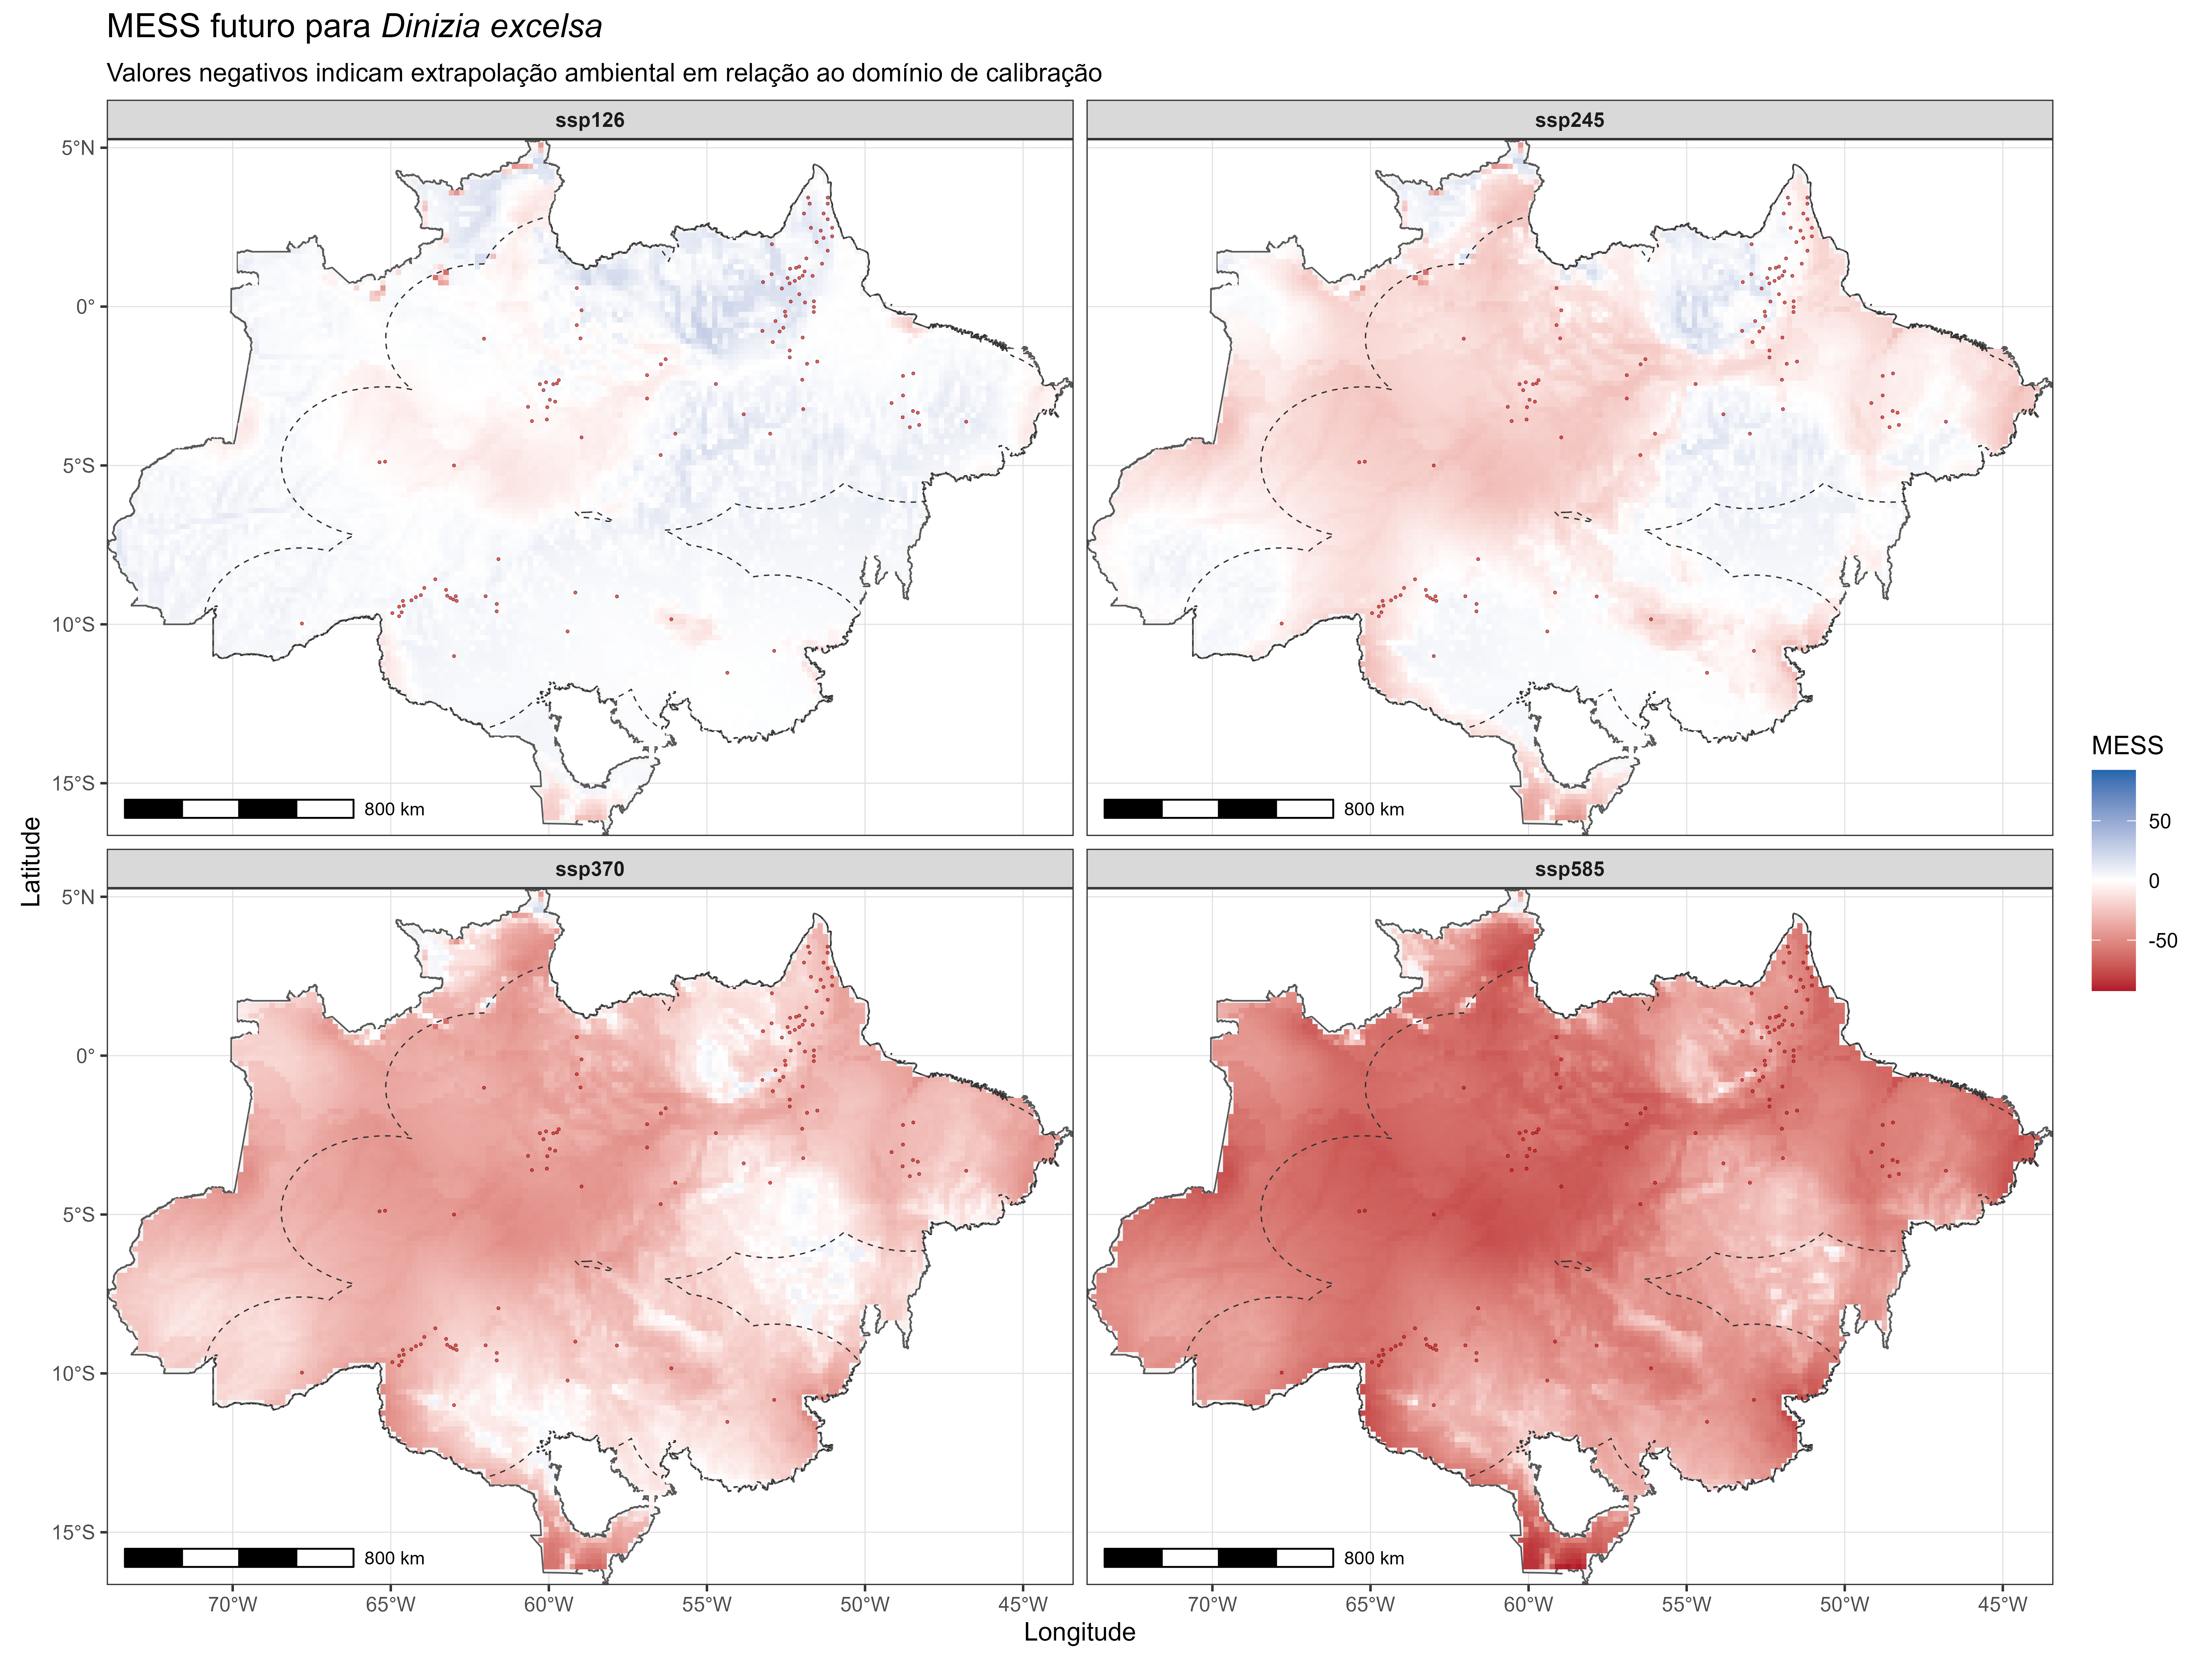
\includegraphics[width=0.96\textwidth]{figuras/unidade14/unidade14_mess_cenarios.png}
\caption{MESS diagnostics for future projections of \textit{Dinizia excelsa}. Negative values identify univariate extrapolation relative to the calibration domain.}
\label{fig:unidade14_mess}
\end{figure}

\section{The most dissimilar variable in MESS}

In addition to the similarity score, MESS can identify the variable contributing the greatest dissimilarity in each cell. This diagnostic helps determine whether future novelty is driven primarily by temperature, precipitation, seasonality, or another predictor. It should not be interpreted as a causal limiting factor for the species; it identifies a statistical boundary of the calibration domain.

\rscriptfile{scripts/unidade14/03_variavel_limitante_mess.R}

\begin{figure}[H]
\centering
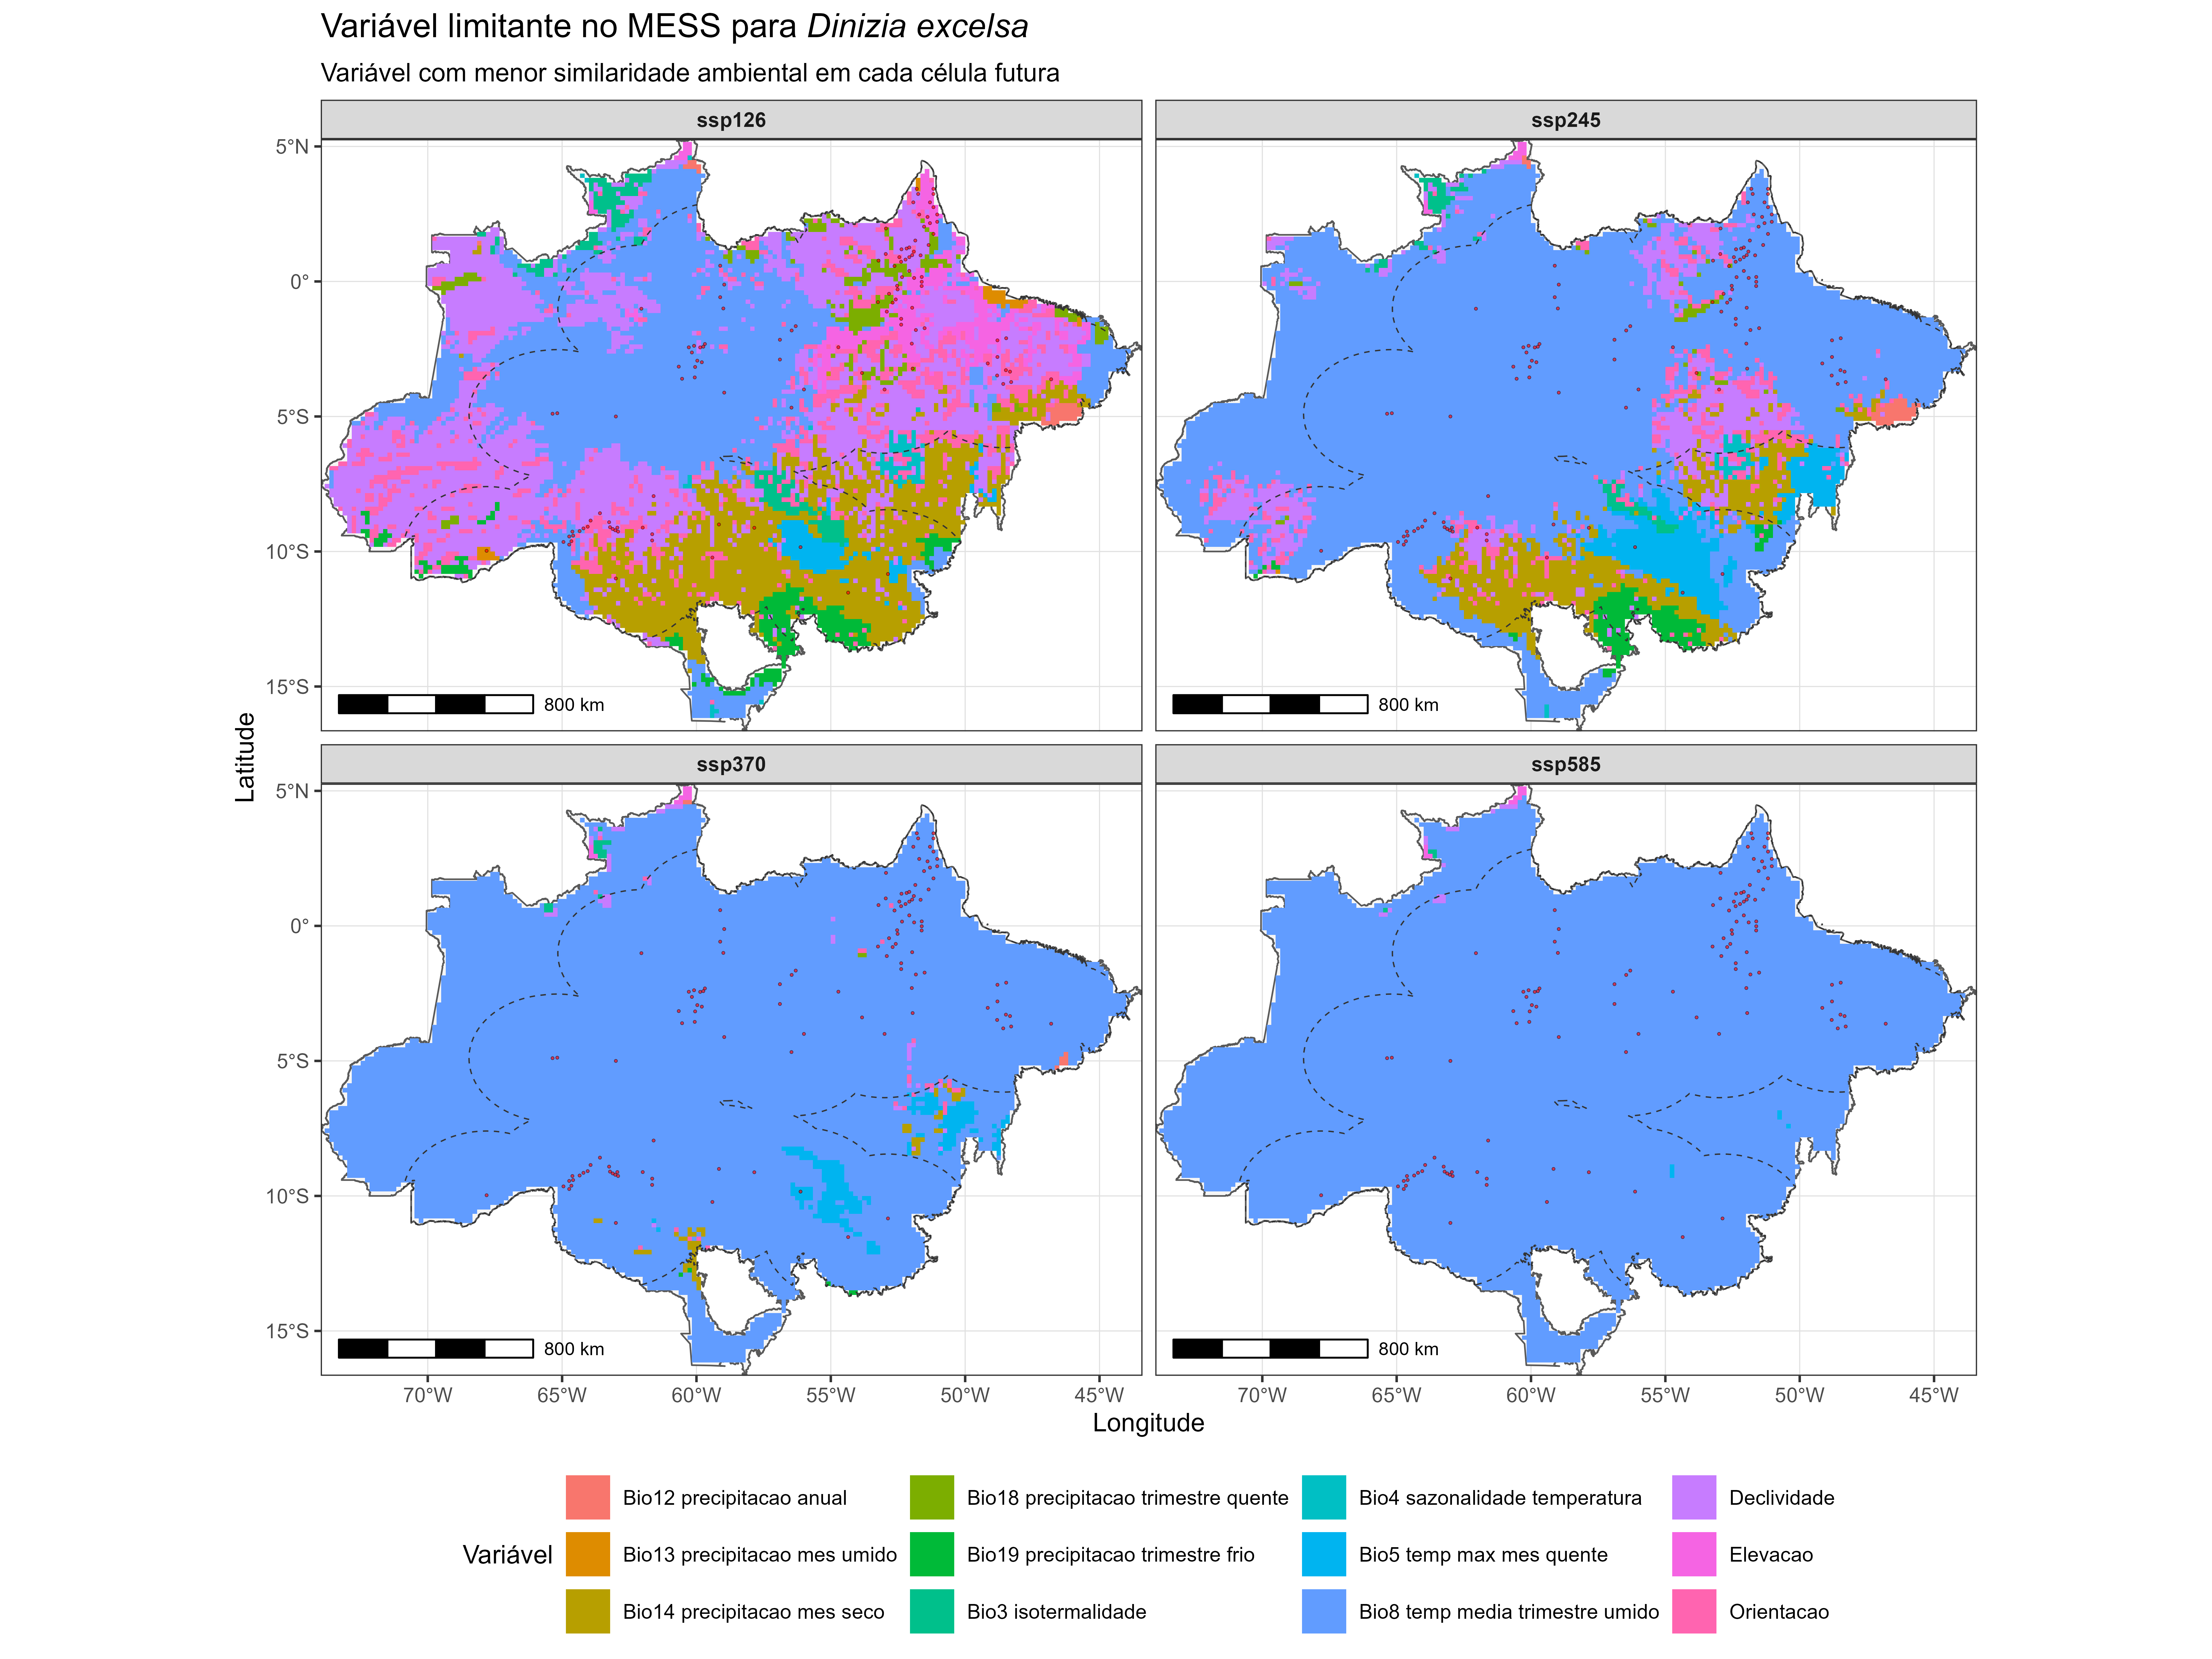
\includegraphics[width=0.96\textwidth]{figuras/unidade14/unidade14_variavel_limitante_mess.png}
\caption{Predictor contributing the greatest environmental dissimilarity in the future MESS diagnostic.}
\label{fig:unidade14_limitante}
\end{figure}

\section{MOP: Mobility-Oriented Parity}

MOP evaluates multivariate environmental similarity between calibration and projection domains using distances in environmental space. It is designed to identify strict extrapolation and to rank similarity among analogous conditions \parencite{owens2013constraints}. Unlike a range-by-range diagnostic, it can reveal novel combinations even when individual predictor values remain within their marginal calibration ranges. Predictor standardization, correlation, reference sampling, and distance definition influence the resulting surface and must be documented.

\rscriptfile{scripts/unidade14/04_calcular_mop_futuro.R}

\begin{figure}[H]
\centering
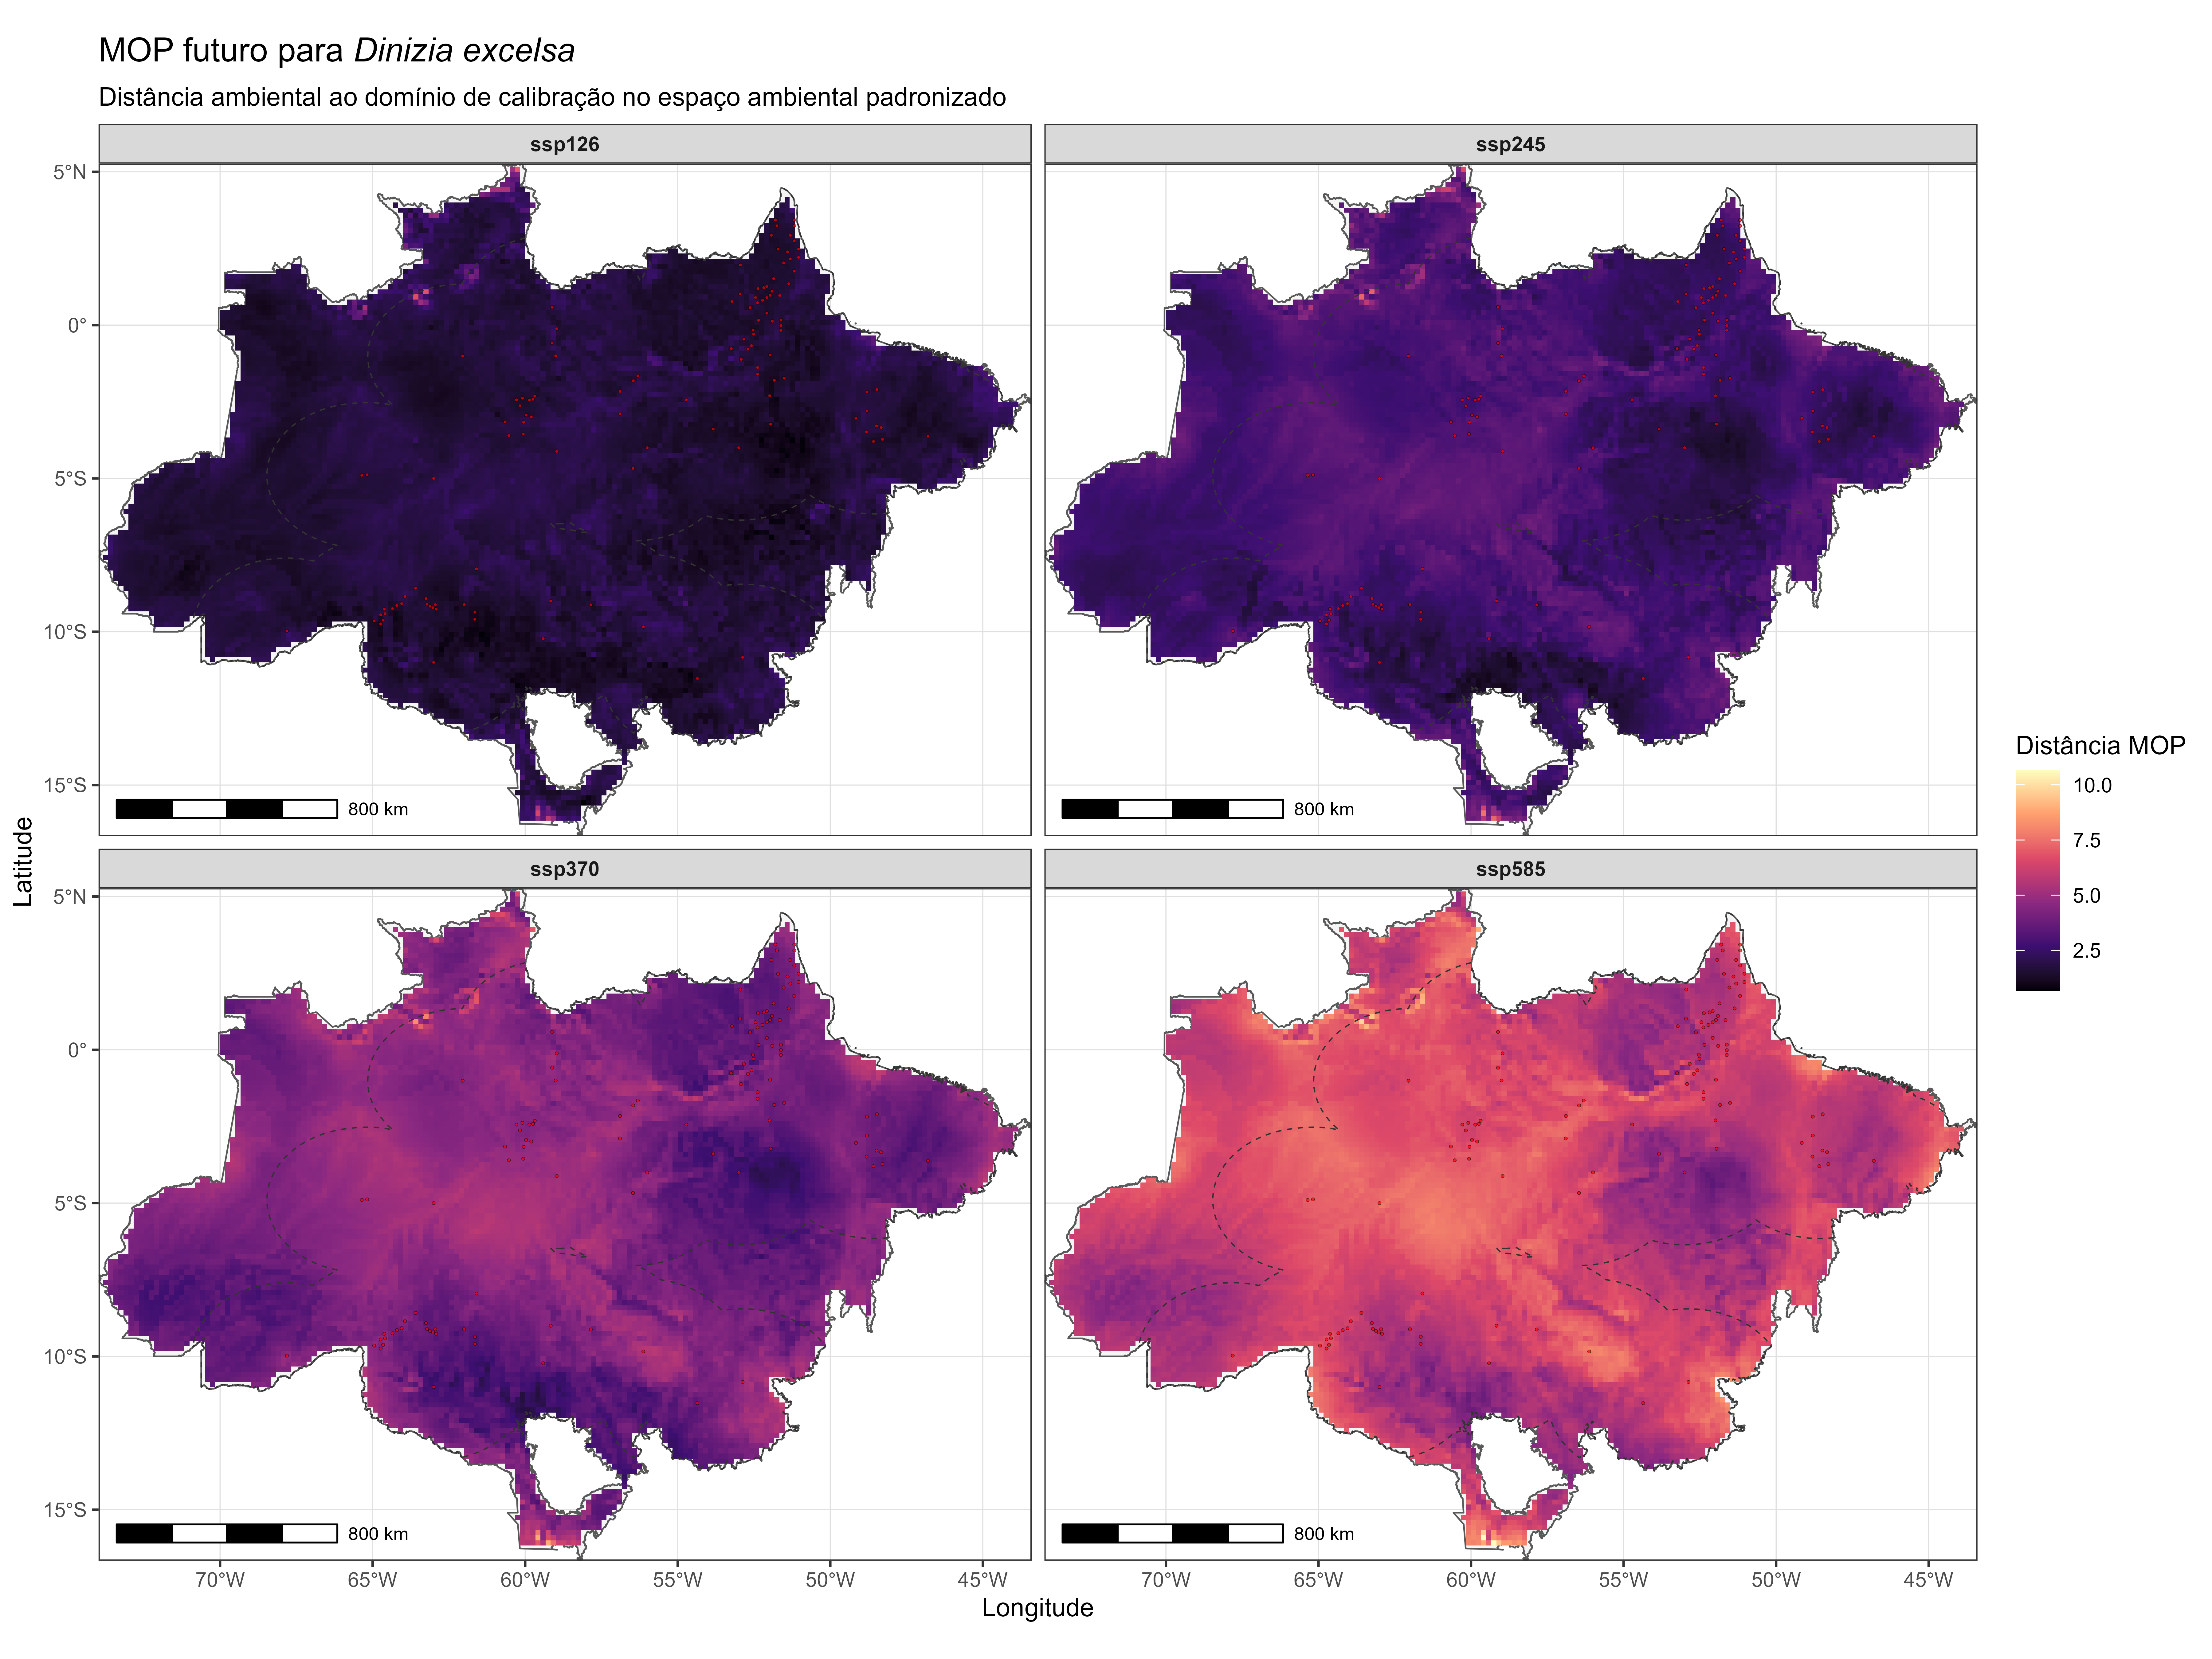
\includegraphics[width=0.96\textwidth]{figuras/unidade14/unidade14_mop_cenarios.png}
\caption{Simplified MOP diagnostics for future scenarios. Under the distance-oriented implementation used here, larger values indicate greater environmental distance from the calibration domain.}
\label{fig:unidade14_mop}
\end{figure}

\begin{atencao}[title={\faExclamationTriangle\quad Verify the direction of the MOP scale}]
MOP software and plotting workflows may express similarity, distance, or rescaled parity in different directions. Always verify the implementation before labeling low or high values as novel; the map legend and methods must state the convention used.
\end{atencao}

\section{Suitability under extrapolation}

Future suitability is now combined with MESS and MOP outputs to locate cells predicted as suitable under novel environmental conditions. Such cells are not necessarily unsuitable, but the evidence supporting their estimates is weaker because the model is being asked to generalize beyond its calibration experience.

\rscriptfile{scripts/unidade14/05_adequabilidade_extrapolacao.R}

\begin{figure}[H]
\centering
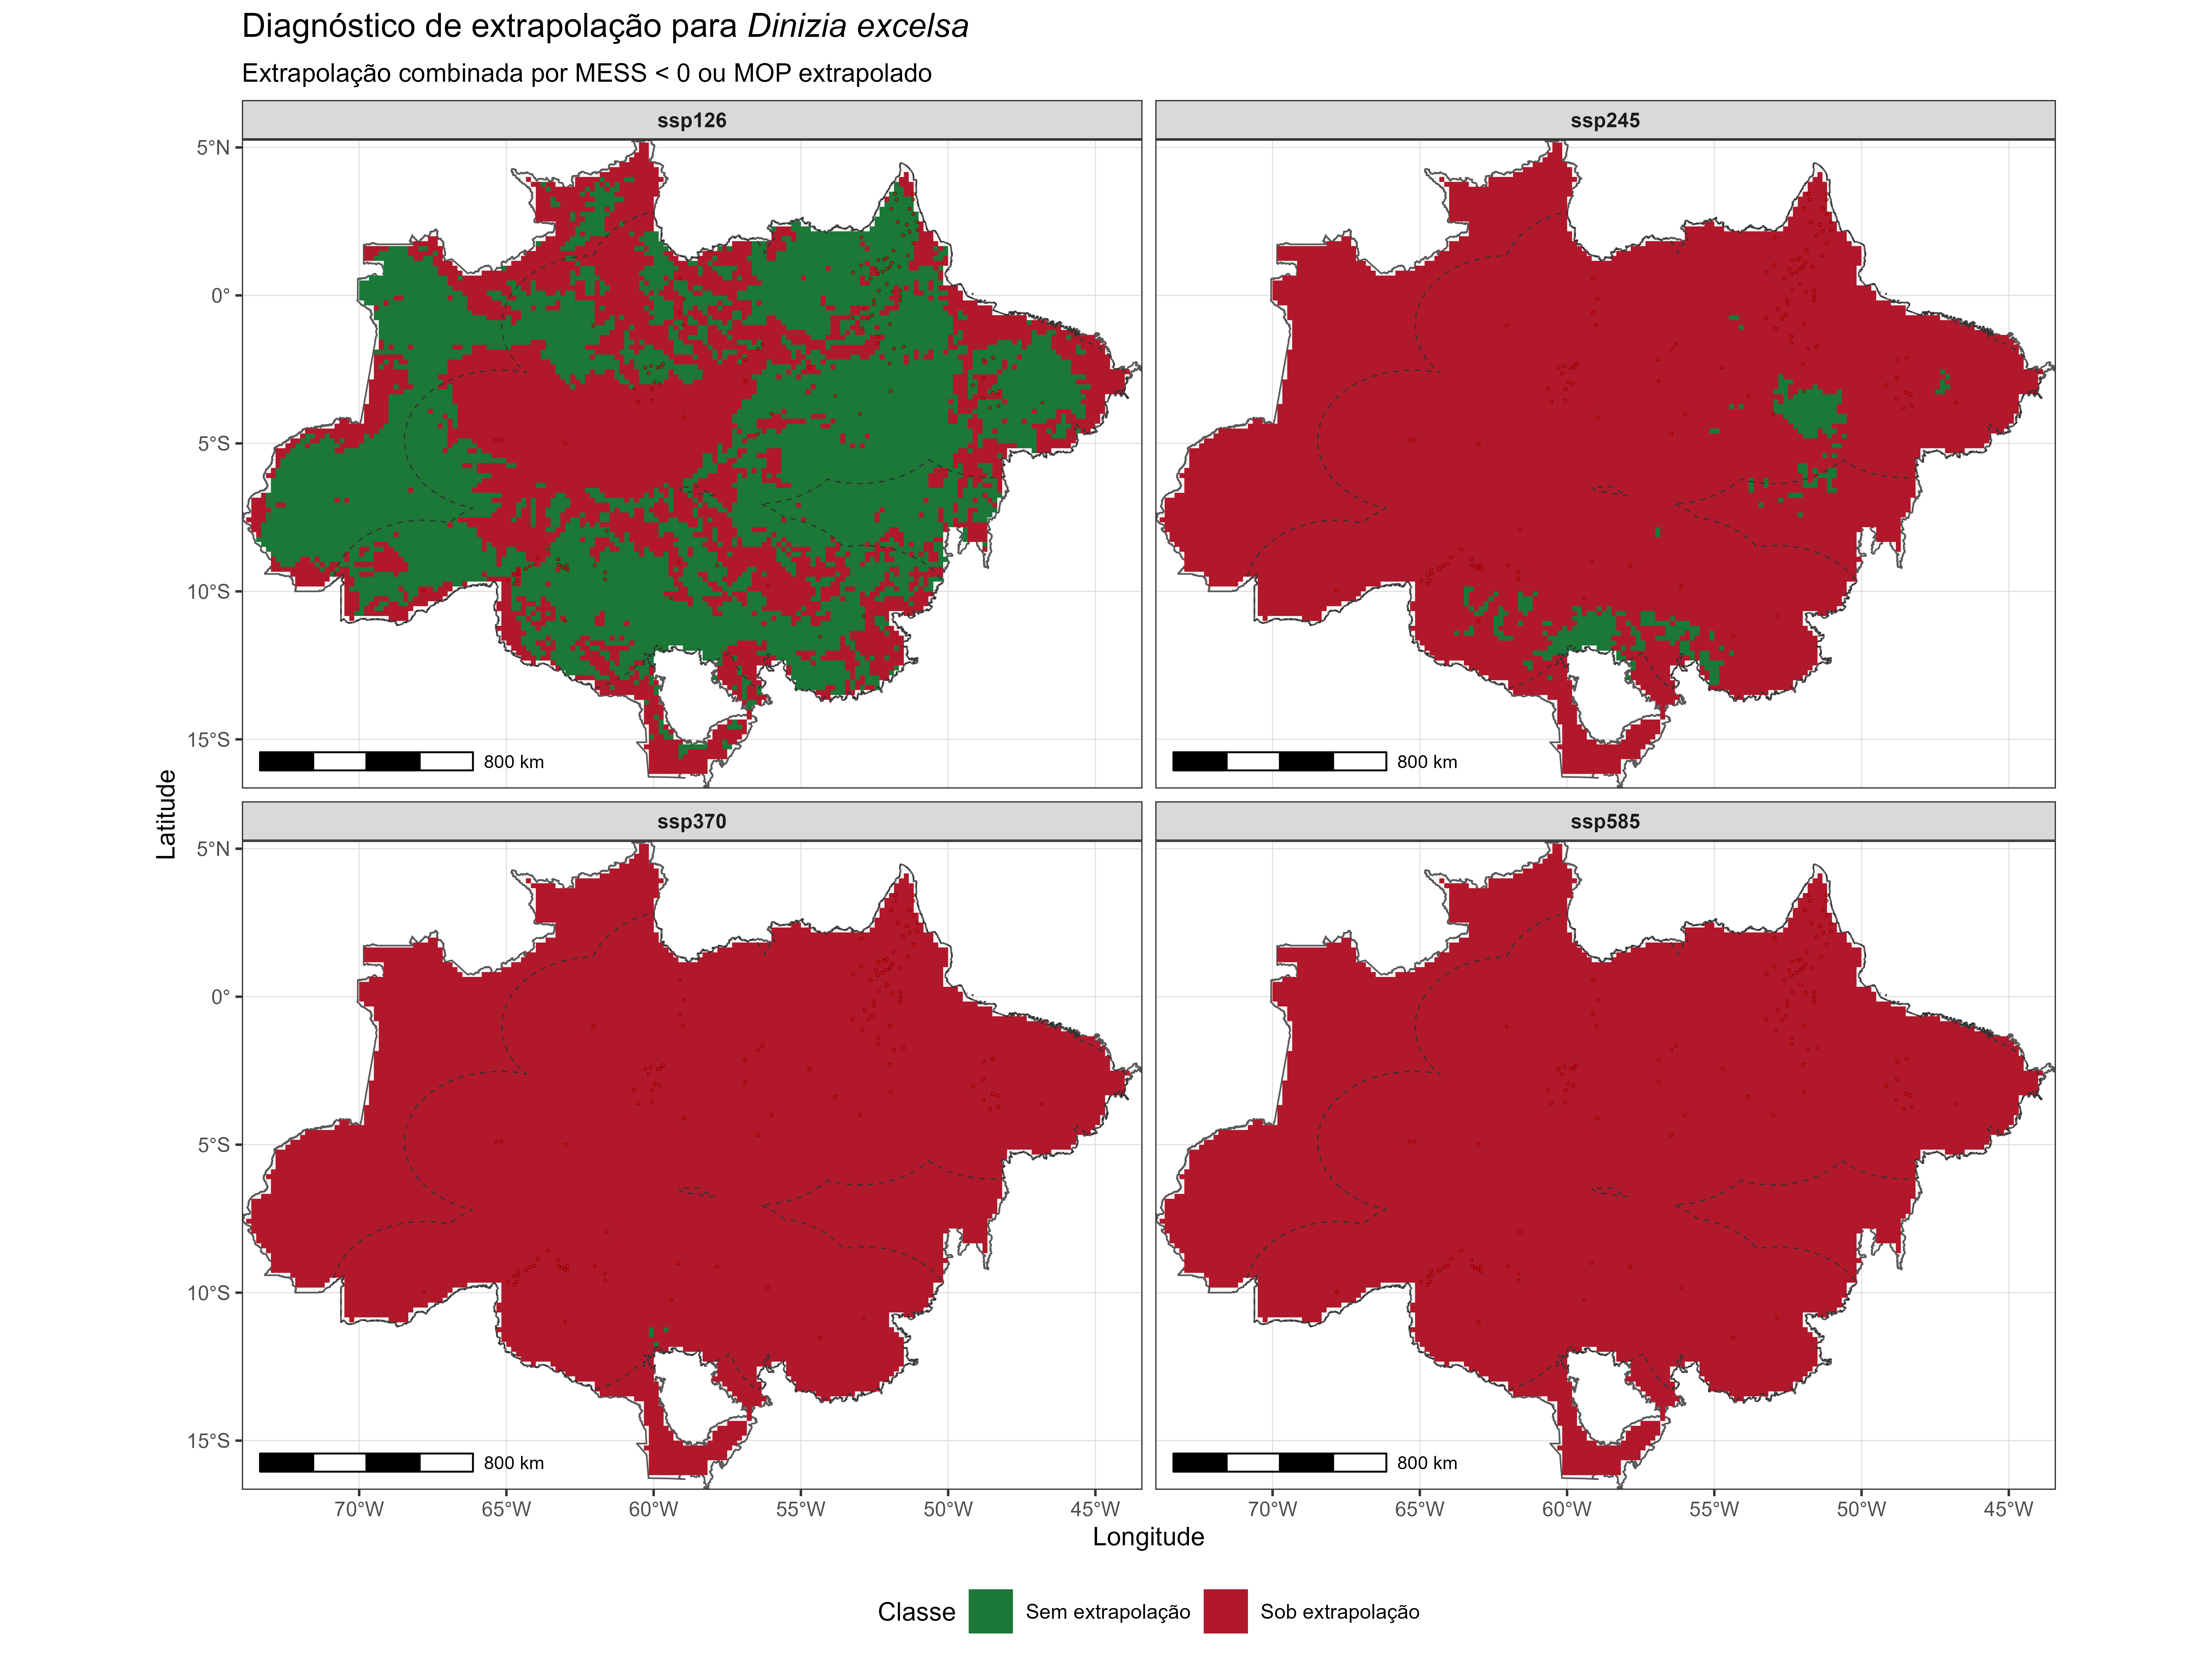
\includegraphics[width=0.96\textwidth]{figuras/unidade14/unidade14_adequabilidade_extrapolacao.png}
\caption{Future suitability combined with diagnostics of environmental extrapolation.}
\label{fig:unidade14_adequabilidade_extrapolacao}
\end{figure}

Novelty masks can be used to flag, summarize, or exclude projections, but these choices answer different questions. Masking prevents unsupported cells from appearing as ordinary predictions; retaining them with prominent uncertainty flags preserves information about where the model is being challenged. The decision should be declared before interpretation and applied consistently.

\section{Synthesis of extrapolation risk}

\rscriptfile{scripts/unidade14/06_sintese_extrapolacao.R}

\begin{figure}[H]
\centering
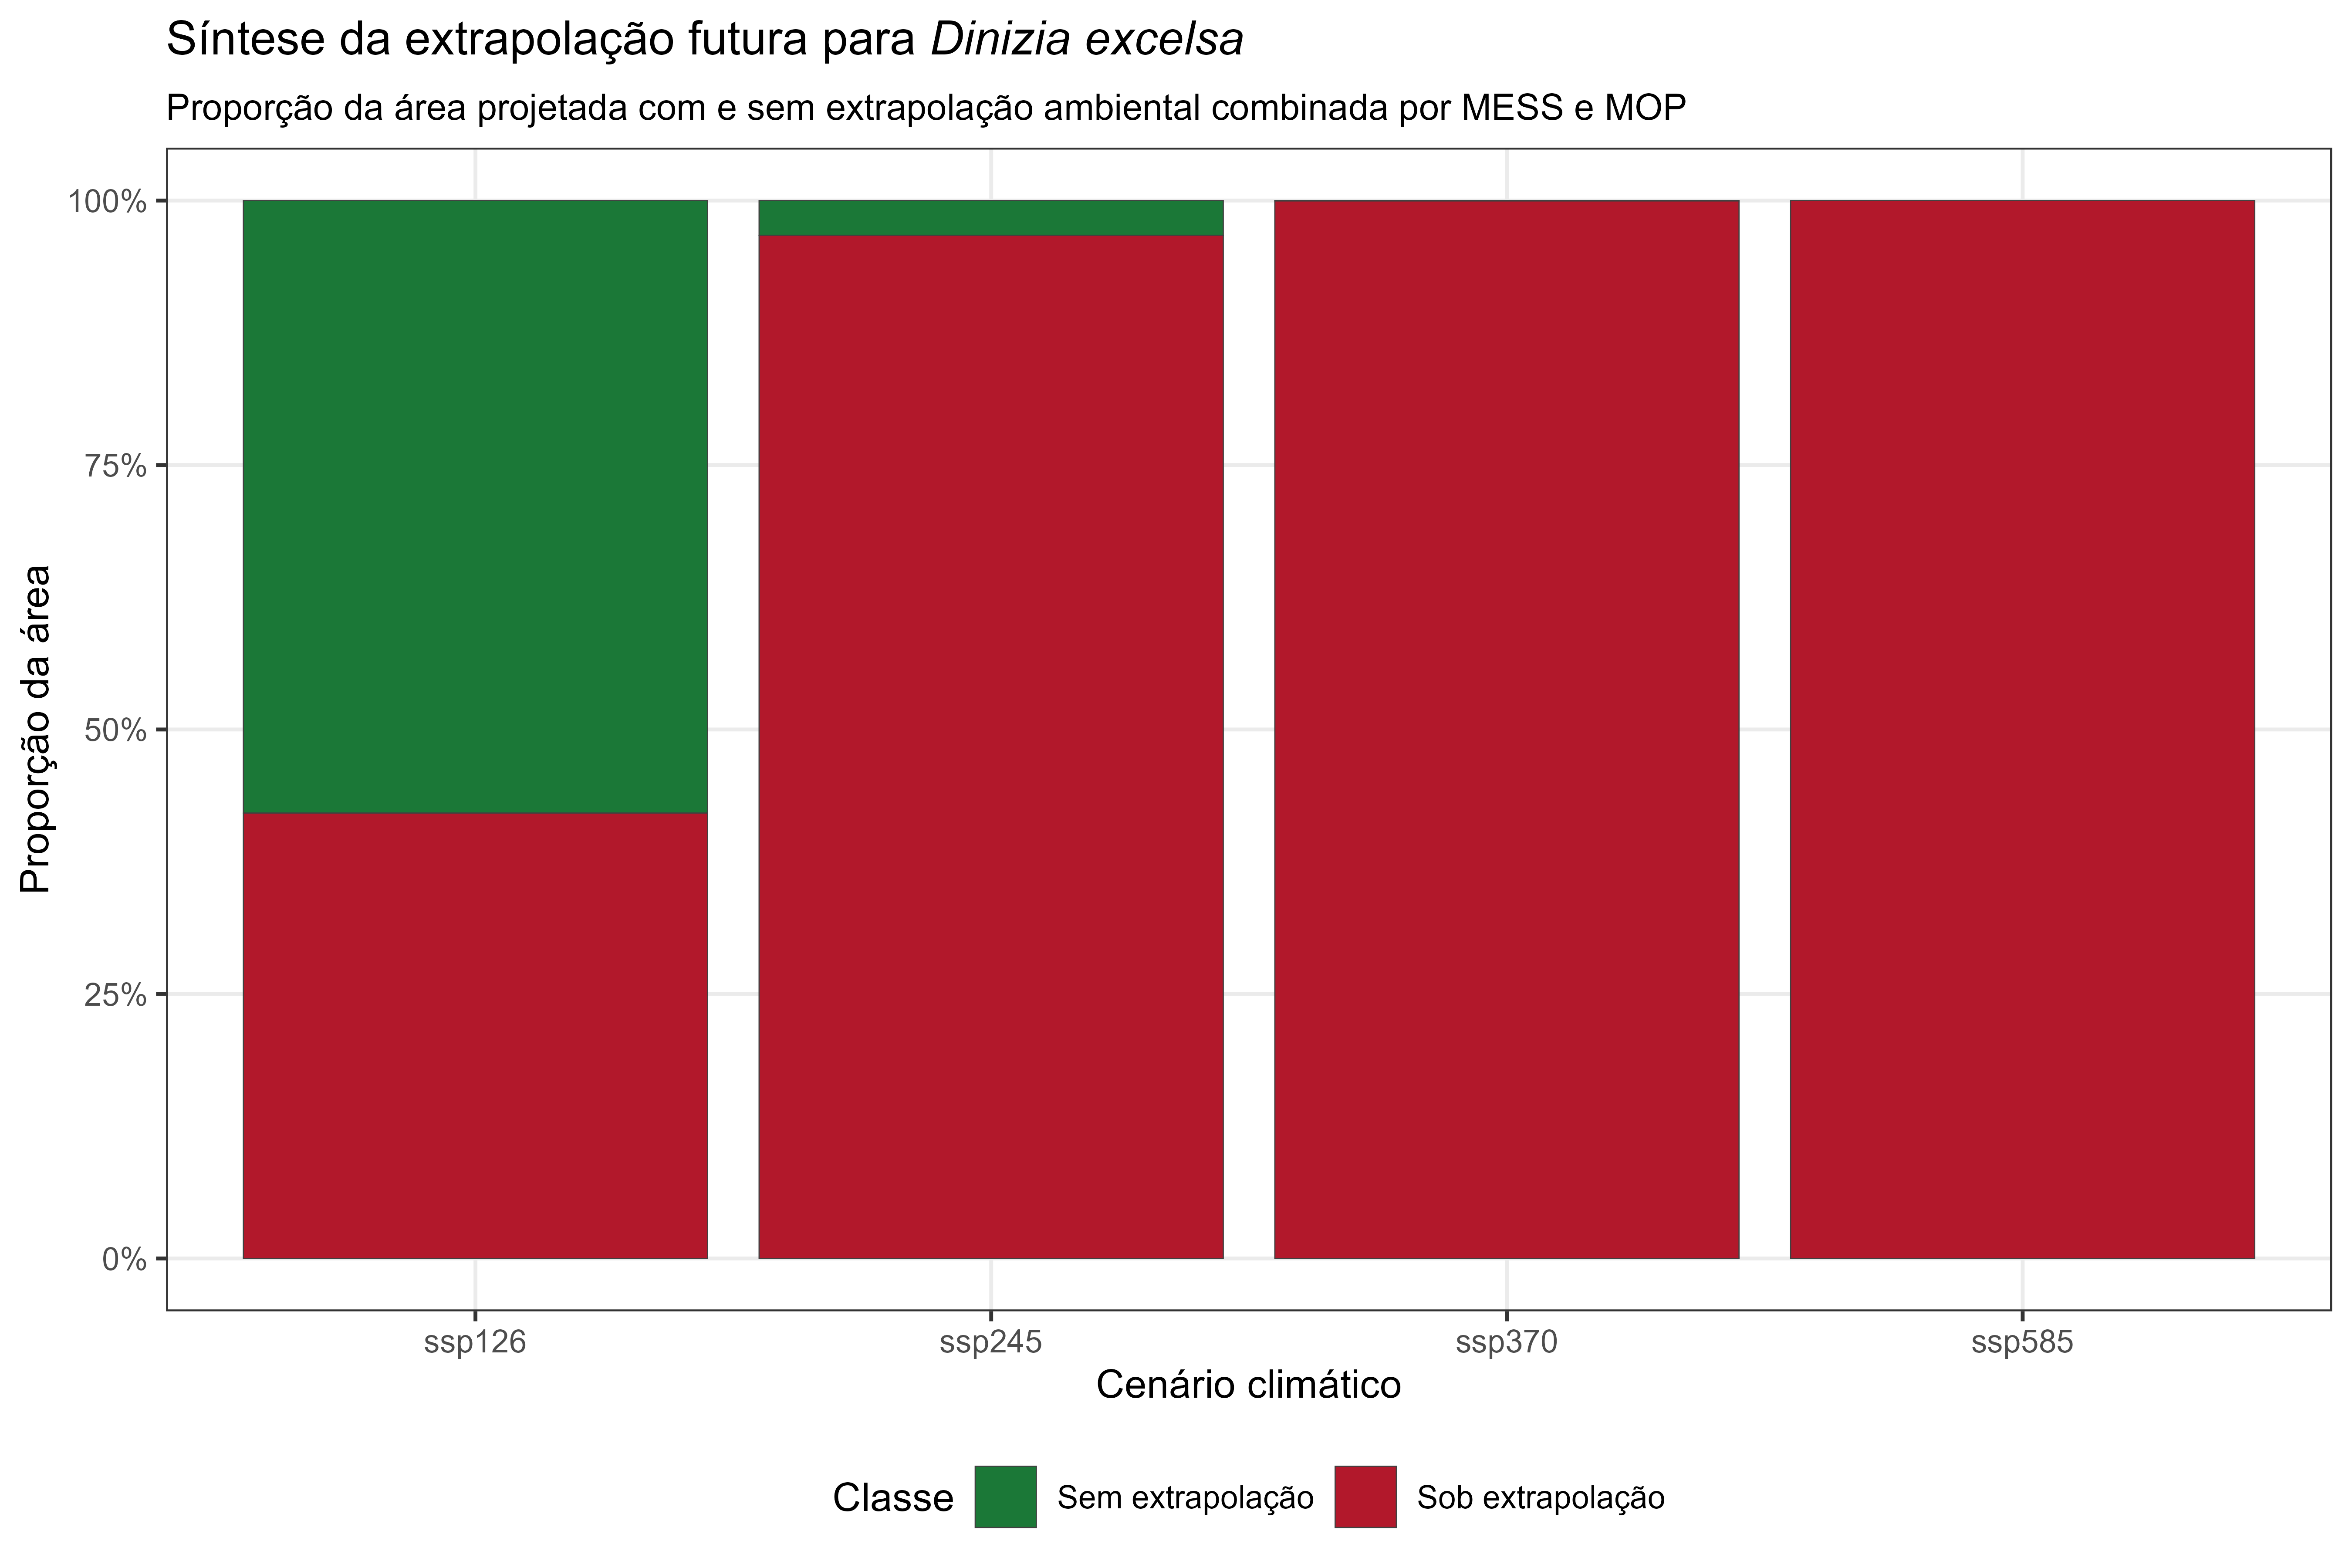
\includegraphics[width=0.88\textwidth]{figuras/unidade14/unidade14_sintese_extrapolacao.png}
\caption{Proportion of the future projection area classified as environmentally extrapolative under each SSP.}
\label{fig:unidade14_sintese}
\end{figure}

The proportion of novel area should be reported relative to an explicit denominator, such as the complete projection extent, the accessible area, or cells classified as suitable. These denominators represent different ecological questions and should not be conflated.

\section{Complete pipeline}

\rscriptfile{scripts/unidade14/07_pipeline_transferencia_extrapolacao.R}

\section{Chapter synthesis}

Spatial and temporal transfer is essential to climate-change and historical SDM applications, but it requires rigorous novelty diagnostics. For \textit{Dinizia excelsa}, MESS and MOP identify environments in which future estimates deserve greater caution. Neither diagnostic measures predictive error directly; instead, they identify departures from the conditions that supported calibration.

\begin{conceito}[title={\faBook\quad Key message}]
Transferred projections are most defensible when environmental novelty is quantified and displayed. High predicted suitability under strong extrapolation is an uncertain hypothesis, not robust evidence of future persistence.
\end{conceito}

\section{Review exercises}

\begin{enumerate}
\item Distinguish environmental interpolation from extrapolation.
\item What does a negative MESS value indicate, and what does a nonnegative value fail to guarantee?
\item How do MESS and MOP differ conceptually?
\item Why can an algorithm predict high suitability in a strongly extrapolative environment?
\item What information should accompany a novelty mask in a published map?
\item Why is temporal transfer particularly sensitive to assumptions about ecological stationarity?
\item How would you combine suitability, MESS, MOP, and dispersal constraints when prioritizing conservation areas?
\end{enumerate}

